

\begin{frame}
\frametitle{Multiple Shooting}
\only<1>{
\begin{figure}
\centering
\includestandalone[width=0.8\textwidth]{TikzMultiShooti1}
\end{figure}
% Bild von Johannes einfügen was Multiple shooting zeigt OHNE Steuerung
}
\only<2>{
\begin{figure}
\centering
\includestandalone[width=0.8\textwidth]{TikzMultiShooti2}
\end{figure}

% Bild von Johannes einfügen was Multiple shooting zeigt MIT Steuerung
}
\only<3>{\begin{figure}
\centering
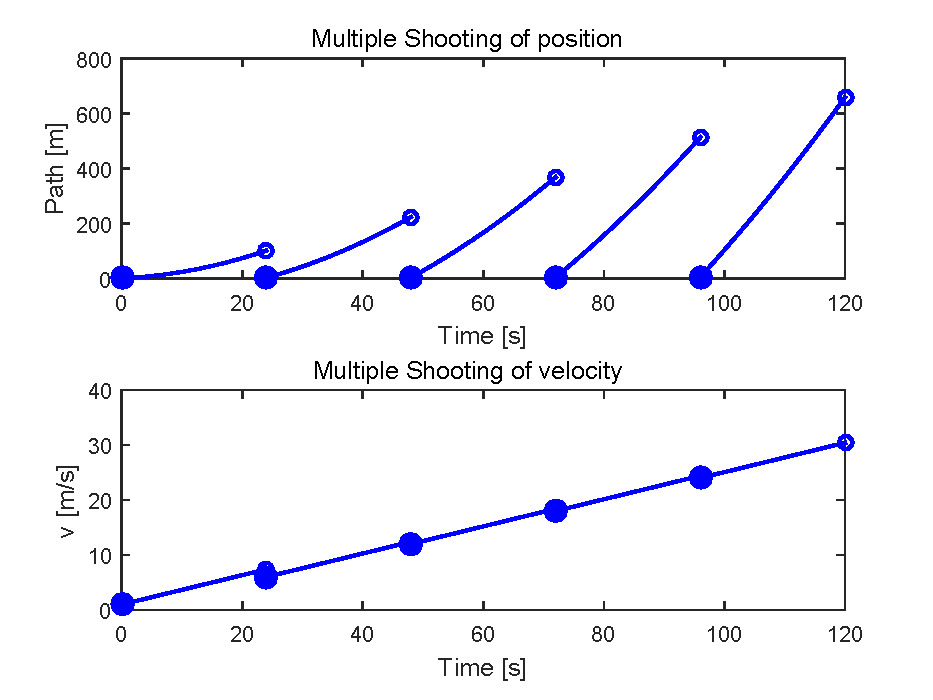
\includegraphics[width=0.9\textwidth]{Sabina/MultipleShooting21.pdf}
\end{figure}}
\only<4>{\begin{figure}
\centering
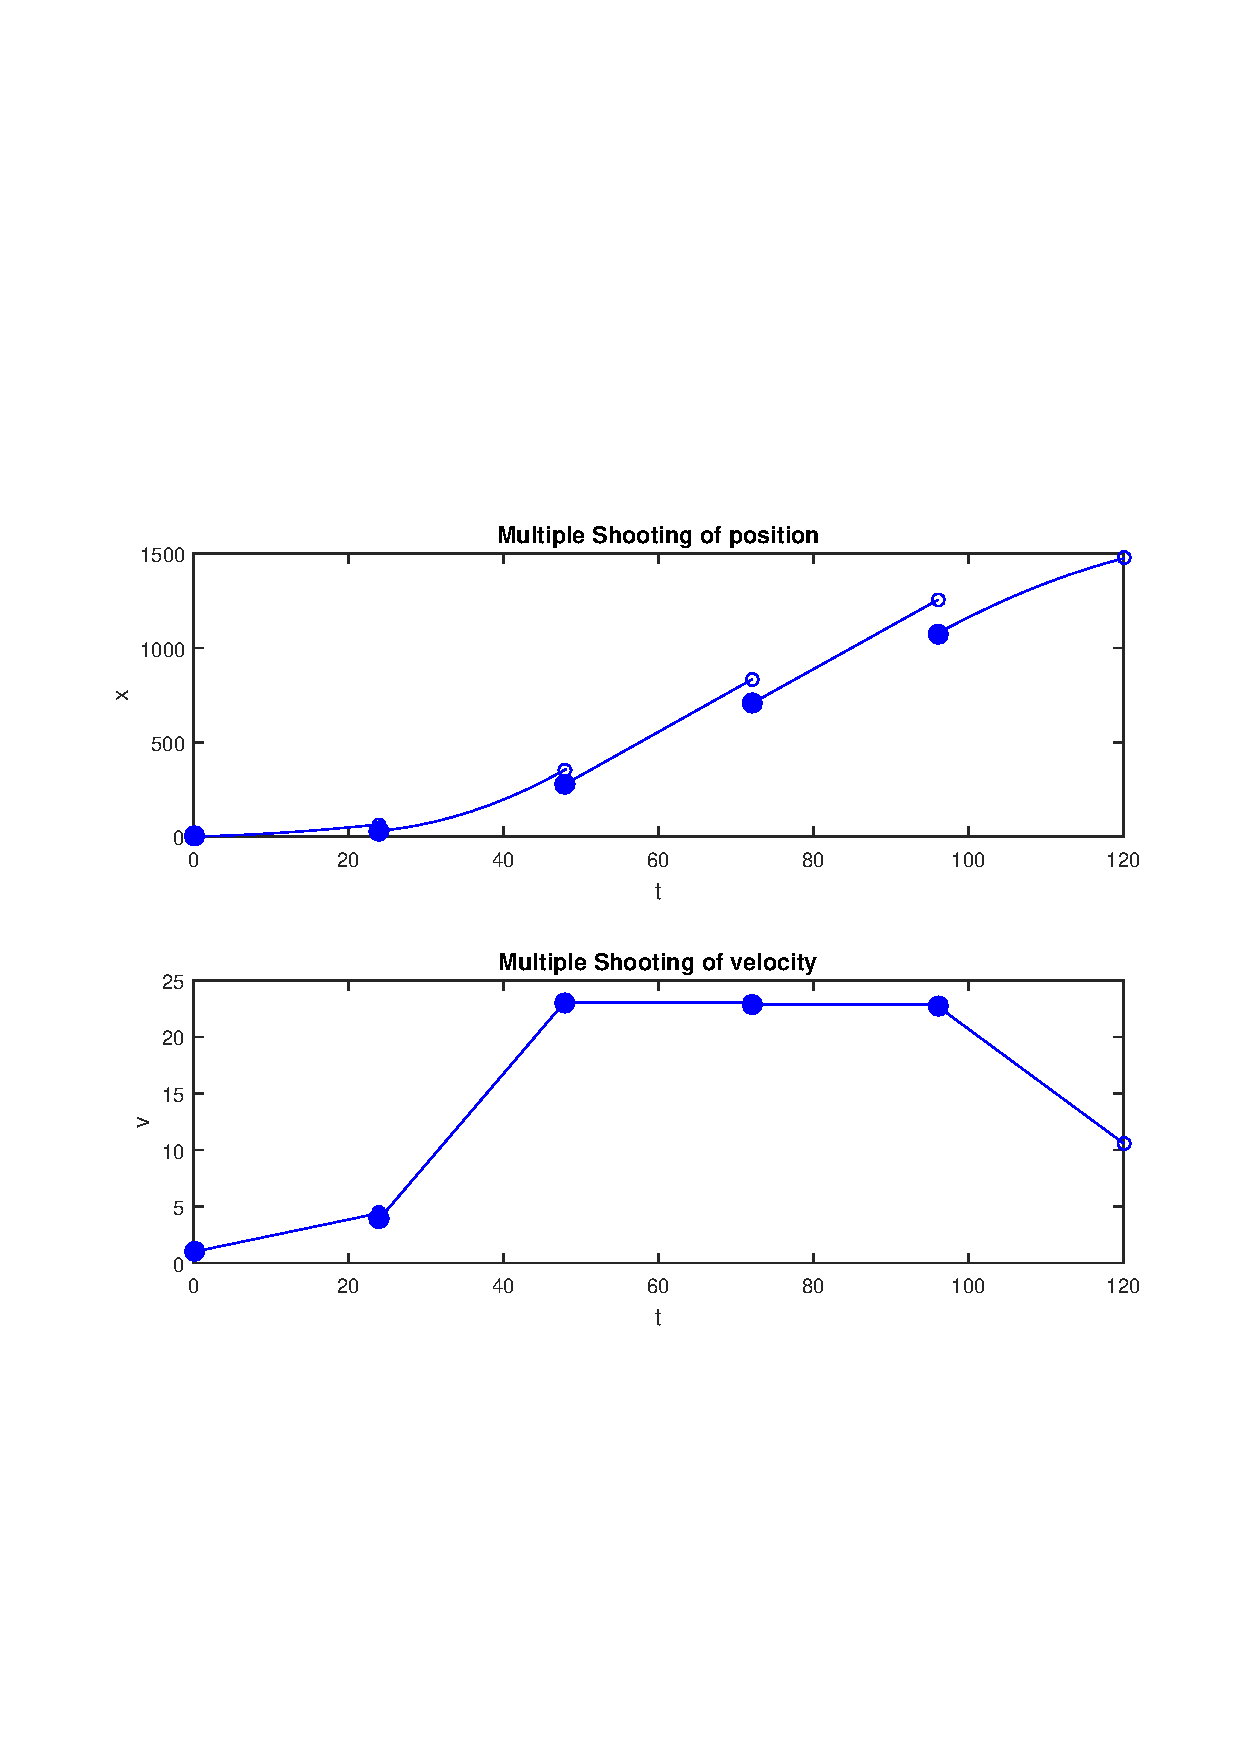
\includegraphics[width=0.9\textwidth]{Sabina/MultipleShooting24.pdf}
\end{figure}}
\only<5>{\begin{figure}
\centering
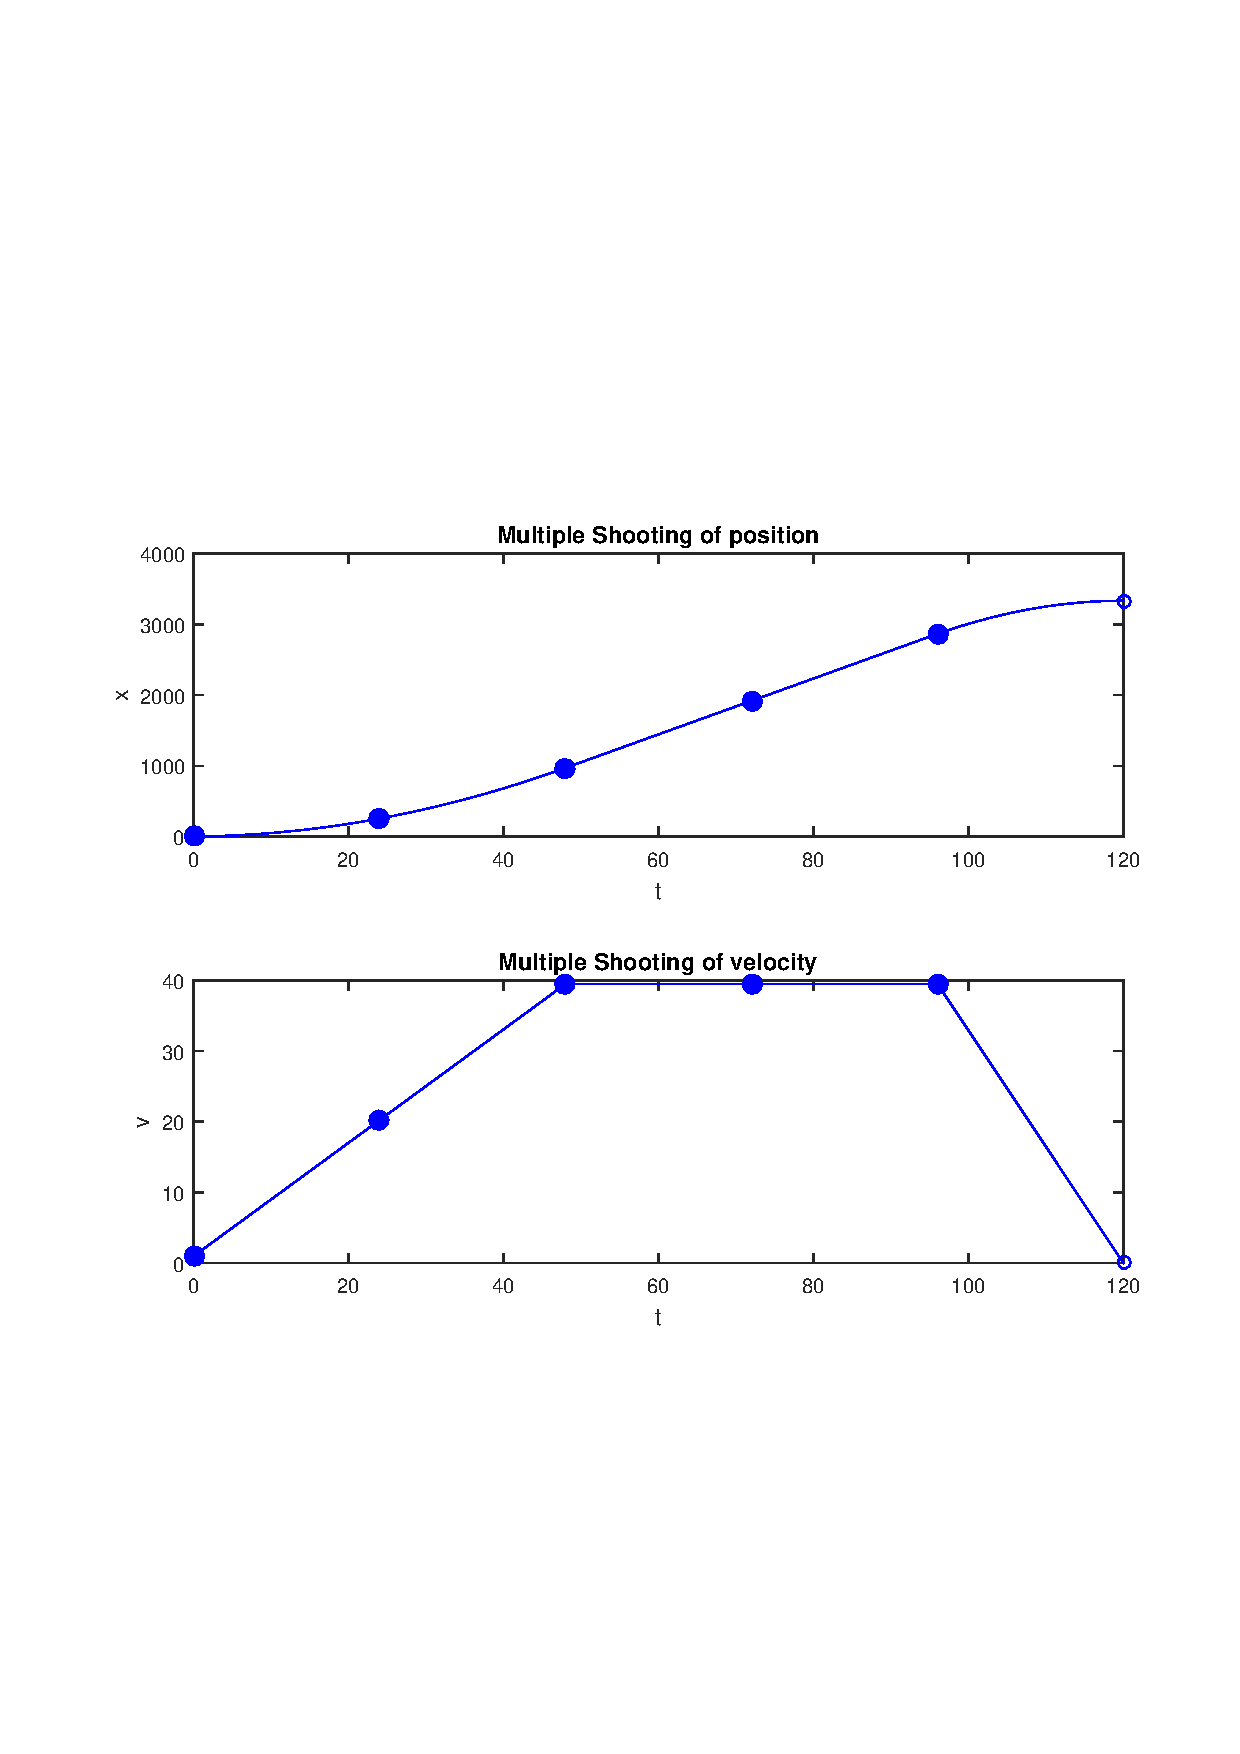
\includegraphics[width=0.9\textwidth]{Sabina/MultipleShooting27.pdf}
\end{figure}}
\only<6>{\begin{figure}
\centering
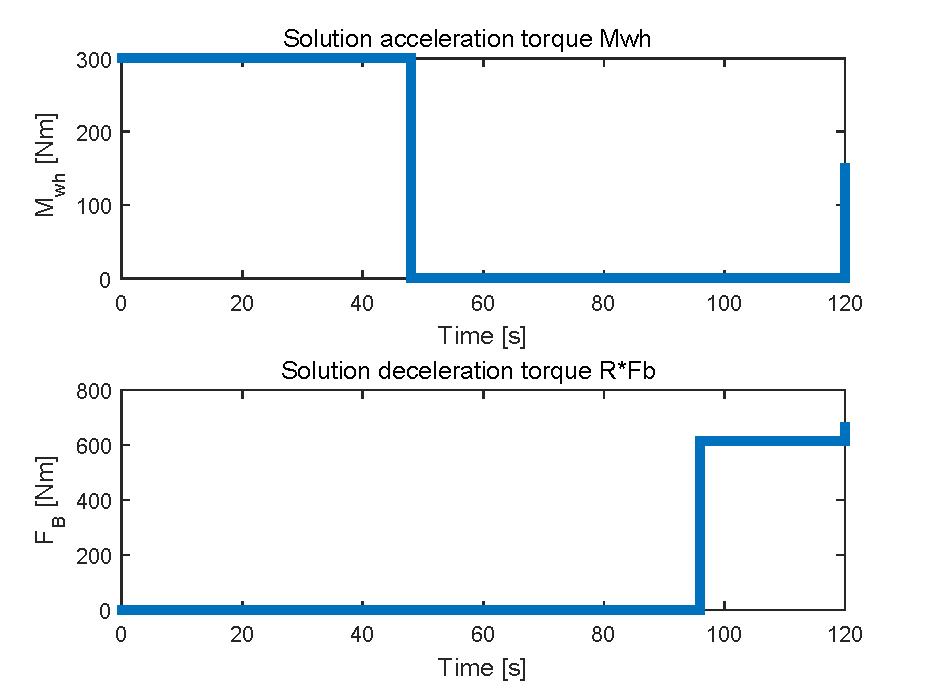
\includegraphics[width=0.9\textwidth]{Sabina/output4.pdf}
\end{figure}}

\note{
\begin{itemize}
\item It might be confusing to plot the state vector as a 1D vector. 
Maybe, it would be better to plot the velocity. I will mention that this is a state
\item The $t$ is above the axis
\item It might be good to add another blue y -axis!
\item The same for the control vector. Is the control between the state by accident?
\item I would not present MATLAB graphics (consistency) - just another tikz graphic with continuous state. 
\item Will the solution output a continuous control? (might be a question of the audience. 
\item I would omit the plots for Mwh and R*Fb. Why are the vertical lines not dashed? (consistency)
\end{itemize}
}

\end{frame}